\documentclass{article}
\usepackage{amsmath,amssymb,amsthm}
\usepackage{listings}
\usepackage{enumerate}
\usepackage{pgfplots}

\title{\textbf{Ordini di calcolo}}
\author{Luca Tagliavini}
\date{February 24-25, 2021}

\begin{document}

\maketitle
\tableofcontents
\pagebreak

\subsection{Modello di calcolo}

Immaginiamo di avere una macchina \emph{a registri} con le seguenti caratteristiche:
\begin{itemize}
  \item La macchina ha $n$ locazioni di memoria, indicizzate da $1$ a $n$
  \item L'accesso in lettura/scrittura richiede sempre \emph{tempo costante}
  \item La macchina ha accesso a operazioni base come somma/moltiplicazione che
    vengono eseguite in \emph{tempo constante}
\end{itemize}

\subsection{Costo computazionale}

Indichiamo con $f(n)$ la quantita' di risorse (tempo, memoria) necessaria al fine
dell'esecuzione di un algoritmo con un input $n$, operante sulla macchina a registri
sopra descritta.

Siamo interessati a studiare \emph{l'ordine di grandezza} di $f(n)$, ignorando
le costanti numeriche o i termini di ordine inferiore. \\
Oltretutto non andremo a quantitifcare un tempo in secondi, ma bensi' il numero
di operazioni elementari svolte dall'algoritmo.

\subsubsection{Esempio}

Consideriamo due algoritmi: $A$ e $B$. Assumiamo le seguenti tempistiche:
\begin{itemize}
  \item $f_A(n) = 10^3n$
  \item $f_B(n) = 10^{-3}n^2$
\end{itemize}

\subsection{Notazione asintitoca $O$ (Omicron)}

Data una funzione $f(n)$ che quantifica il costo di un algoritmo con input n, usiamo
$O(f(n))$ per indicare l'insieme di funzioni $g(n)$ che al limite stanno sempre sotto $f(n)$, ovvero. 
\begin{align*}
g(n) \in O(f(n)) \text{ quando } \exists c > 0, n_0 \geq 0. \forall n \geq n_0. \qquad g(n) \leq c \cdot f(n)
\end{align*}

\begin{quote}
  Esiste un $n_0$ dopo il quale la funzione $g$ rimane inferiore rispetto a $f$.
  $c$ e' una costante che eventualmente devo applicare a $f$ per renderla \emph{sempre} maggiore di $g$.
  Abuso di notazione: $g = O(f(n))$ come $g \in O(f(n))$.
\end{quote}

Esempio dove si ha $g(n) \in O(f(n))$, scegliendo $n_0 = 2.15, c = \frac{1}{4}$

\begin{center}
\begin{tikzpicture}
\begin{axis}[
  axis lines = box,
  xlabel = $n$,
  ytick={100},
  xtick={2.15},
  xmajorgrids=true,
  grid style=dashed,
]

\addplot [
  domain=1:3.5, 
  samples=250, 
  color=magenta,
]{1/4 * e^x};
\addlegendentry{$\frac{1}{4} \cdot e^n \quad (c \cdot f)$}

\addplot [
  domain=1:3.5, 
  samples=250, 
  color=orange,
]{x};
\addlegendentry{$n \quad (g)$}

\end{axis}
\end{tikzpicture}
\end{center}

\subsection{Operazione asintotica $\Omega$ (Omega)}

Data una funzione $f(n)$ che quantifica il costo di un algoritmo con input n, usiamo
$\Omega(f(n))$ per indicare l'insieme di funzioni $g(n)$ che al limite si stanno sempre sopra $f(n)$, ovvero. 
\begin{align*}
g(n) \in \Omega(f(n)) \text{ quando } \exists c > 0, n_0 \geq 0. \forall n \geq n_0. \qquad g(n) \geq c \cdot f(n)
\end{align*}

Esempio dove si ha $g(n) \in \Omega(f(n))$, scegliendo $n_0 = 8.61, c = \frac{1}{4}$

\begin{center}
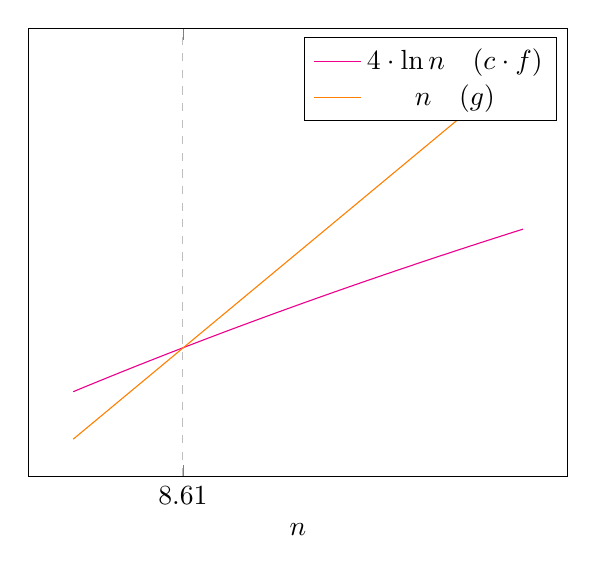
\begin{tikzpicture}
\begin{axis}[
  axis lines = box,
  xlabel = $n$,
  ytick={100},
  xtick={8.61},
  xmajorgrids=true,
  grid style=dashed,
]

\addplot [
  domain=8:10.5, 
  samples=250, 
  color=magenta,
]{4 * ln(x)};
\addlegendentry{$4 \cdot \ln{n} \quad (c \cdot f)$}

\addplot [
  domain=8:10.5, 
  samples=250, 
  color=orange,
]{x};
\addlegendentry{$n \quad (g)$}

\end{axis}
\end{tikzpicture}
\end{center}

\subsection{Operazione asintotica $\Theta$ (Theta)}

Data una funzione $f(n)$ che quantifica il costo di un algoritmo con input n, usiamo
$\Theta(f(n))$ per indicare l'insieme di funzioni $g(n)$ che al limite si comportano come $f(n)$, ovvero. 
\begin{align*}
g(n) \in \Theta(f(n)) \text{ quando } \exists c_1 > 0, c_2 > 0, n_0 \geq 0. \forall n \geq n_0. \\
c_1 \cdot f(n) \leq g(n) \leq c_2 \cdot f(n)
\end{align*}

\begin{quote}
  Le funzioni $g$ e $f$ crescono esattamente con lo stesso ordine di grandezza.
  Ossia due funzioni espresse in polinomi saranno in relazione $\Theta$ sse il polinomio di grado maggiore e' lo stesso.
\end{quote}

Esempio dove si ha $g(n) \in \Theta(f(n))$, scegliendo $n_0 = 1, c_1 = 6, c_2 = \frac{3}{2}$

\begin{center}
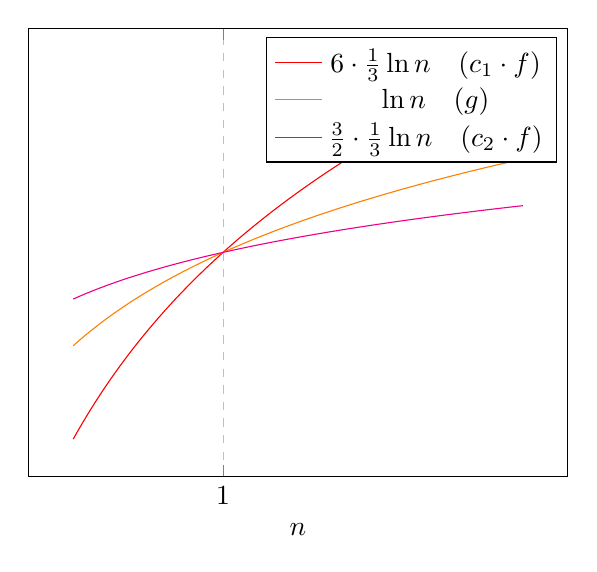
\begin{tikzpicture}
\begin{axis}[
  axis lines = box,
  xlabel = $n$,
  ytick={100},
  xtick={1},
  xmajorgrids=true,
  grid style=dashed,
]

\addplot [
  domain=0.5:2, 
  samples=250, 
  color=red,
]{2 * ln(x)};
  \addlegendentry{$6 \cdot \frac{1}{3}\ln{n} \quad (c_1 \cdot f)$}

\addplot [
  domain=0.5:2, 
  samples=250, 
  color=orange,
]{ln(x)};
\addlegendentry{$\ln{n} \quad (g)$}

\addplot [
  domain=0.5:2, 
  samples=250, 
  color=magenta,
]{1/2 * ln(x)};
\addlegendentry{$\frac{3}{2} \cdot \frac{1}{3}\ln{n} \quad (c_2 \cdot f)$}

\end{axis}
\end{tikzpicture}
\end{center}

\subsection{Teoremi}

\begin{itemize}
  \item \textbf{simmetria}: $g(n) = \Theta(f(n))$ sse $f(n) = \Theta(g(n))$
  \item \textbf{simmetria trasposta}: $g(n) = O(f(n))$ sse $f(n) = \Omega(g(n))$
  \item \textbf{transitivita'}: $g(n) = O(f(n)) \wedge f(n) = O(h(n))$ allora $g(n) = O(h(n))$. \\
        Lo stesso vale per $\Theta$ e $\Omega$.
\end{itemize}

\subsection{Tabella degli ordini di grandezza}

\begin{center}
\begin{tabular}{ |c|c|c| } 
  \hline
  $O(f(n))$ & Ordine & Esempio \\
  \hline\hline
  $O(1)$ & costante & numero pari, somma, moltiplicazione \\ 
  \hline
  $O(\log n)$ & logaritmico & ricerca binaria (array ordinato) \\ 
  \hline
  $O(n)$ & lineare & ricerca in un array disordinato \\ 
  \hline
  $O(n \log n)$ & pseudo-lineare & ordinamento di un array (merge sort) \\ 
  \hline
  $O(n^2)$ & quadratico & ordinamento di un array (bubble sort) \\ 
  \hline
  $O(n^3)$ & cubico & prodotto di due matrici $n \times n$ \\ 
  \hline
  $O(c^n)$ & esponenziale, $c > 1$ & \emph{subset-sum problem} con forza bruta \\ 
  \hline
  $O(n!)$ & fattoriale & \emph{commesso viaggiatore} con forza bruta \\ 
  \hline
  $O(n^n)$ & esponenziale, base $n$ & \emph{$n$-queens} tramite forza bruta \\ 
  \hline
\end{tabular}
\end{center}

\begin{quote}
  \begin{itemize}
    \item \textbf{subset-sum}: abbiamo un insieme di numeri, dobbiamo trovare un sottoinsieme al quale, applicando
      una sommatoria si ottiene un valore desiderato. L'approccio forza bruta considera \emph{ogni sottoinsieme possibile}.
    \item \textbf{commesso viaggiatore}: abbiamo una mappa e delle strade (rappresentate con grafi) e vogliamo trovare il modo
      migliore per il commesso di viaggiare da A a B. L'approccio forza bruta consiste nel valutare \emph{ogni strada possibile}.
    \item \textbf{n-queens}: problema che ci chiede di porre le regine in una scacchiera $n \times n$ in modo
      che esse non si mangino a vicenda. L'approccio forza bruta prova \emph{ogni possibile combinazione} di piazzamento in $n \times n$.
  \end{itemize}
\end{quote}

\subsection{Spiegazione di alcuni ordini di grandezza}

\begin{itemize}
  \item \textbf{binary serach}: Andiamo ad analizzare gli elementi dell'array considerando meta' array alla volta,
    partendo da $n$ elementi, guardando poi $\frac{n}{2}$,  poi $\frac{n}{4}$ e cosi' via. Facendo questa procedura
    si svolgono $\log n$ (dove $\log$ e' sempre $\log_2$ in algoritmi). Eccone una spiegazione:
    \begin{align*}
      \frac{n}{2} \longrightarrow &\frac{n}{4} \longrightarrow \frac{n}{8} \\
      \text{fino ad arrivare ad} & \text{ avere una frazione che vale 1} \\
      1 &= \frac{n}{2^{\#}} \\
      2^{\#} &= n \\
      \# &= \log_2{n}
    \end{align*}

  \item \textbf{merge sort}: Analizziamo gli array a meta' come nelle binary
    search, e ogni operazione di ordinamento sulle sottoparti richiede $O(\frac{n}{2})$
    tempo per svolgere i confronti; Visto che dovremo ordinare entrambe le meta' dell'array,
    svolgeremo $O(\frac{n}{2}) \cdot 2$ volte l'operazione di ordinamento, ovvero $O(n)$. \\
    Il che ci da un costo di $O(n) \cdot O(\log n) = O(n \log n)$
\end{itemize}

\subsection{Confronto con limite}

Per confrontare l'ordine di grandezza asintotica di due funzioni $g(n)$ e $f(n)$, si puo' svolgere il:
\begin{align*}
  \lim_{n \rightarrow \infty}{\frac{g(n)}{f(n)}} = 
\end{align*}
\begin{itemize}
  \item $\infty$: $g(n) = \Omega(f(n))$ poiche' $g(n)$ ha una crescita superiore
  \item $k \in \mathbb{R}$: $g(n) = \Theta(f(n))$ poiche' $g(n)$ cresce come $f(n)+k$
  \item $0$: $g(n) = O(f(n))$ poiche' $g(n)$ ha una crescita inferiore
\end{itemize}

\end{document}
